\chapter{Literature Review}\label{Literature Review}

\section{The Media}

\subsection{Role of the Media in a crisis}\label{Role of the Media in a crisis}

TODO

\subsection{French Press}\label{chap:French Press}

TODO: possibly include some history of french press, AFP and more
% Find what the role of the press is, should be specifically in the context of important, hurtful events
%How the people see the covid 19 pandemic

\section{Sentiment Analysis}\label{Sentiment Analysis}

TODO: detail sections on lexicon / ml, lemmatization vs stemming and more (note: may be worth mentioning regexp)

\subsection{TODO}

%\subsection{Lemmatization}
\label{lemmatization}

%compare treetagger and SpaCy -- show mean scores.
% look into ML vs Lexicon, stemming vs lemmas
% look into language issue English vs others
% french dictionaries

\section{French Lexicons}\label{French Lexicons}

\subsection{FEEL}\label{chap: feel}

TODO

\subsection{Diko}\label{chap: diko}

TODO

\subsection{Polarimots}\label{chap: polarimots}

TODO

\section{Statistical Methods}\label{Statistical Methods}

Statistical methods represents a key focus for this thesis, as specified in the research objectives (Chapter \ref{chap: Research Objectives}). It provides the link between observed values and identifying potential relationships. The various statistical methods used throughout this thesis will be introduced in the following sections.

\subsection{Core Statistics}

This first section introduces key, core statistic measures which are used throughout this thesis.

\subsubsection{Mean}

The mean is a very well known statistical measure with consists of the sum of the deviation of all of the numbers in a sample by the size of that sample. In other words, it is the average value in a sample. It is commonly referred to as $\bar{x}$ for a sample as well as $\mu$ for a population. It can be written as such:

\begin{equation}
    \mu = \bar{x} = \frac{1}{N}\sum^{N}_{i=1} x_{i}
\end{equation}
Where N is the sample size and $x_{i}$ represents the ith value in the sample.

\subsubsection{Variance and Standard Deviation}

The standard deviation and variance are related. A common symbol for the standard deviation is $\sigma$ for a population and $S$ for a sample. Given the standard deviation $S$ or $\sigma$ then the variance is its squared value: $S^{2}$ or $\sigma^{2}$.

The standard deviation measures how much data diverges from the mean. A low value indicates that the data is clustered around the mean, on the other hand a high standard deviation indicates that the sample is more spread out. The variance also measures how distributed data is relative to the mean in the same manner, except in much larger values as it is squared.

The mathematical formula for computing the standard deviation and variance for a sample is the following:
\begin{equation}
    S = \sqrt{\frac{\sum_{i=1}^{N}(x_{i} - \bar{x})^{2}}{N - 1}}
\end{equation}
\begin{equation}
    S^2 = \frac{\sum_{i=1}^{N}(x_{i} - \bar{x})^{2}}{N - 1}
\end{equation}

\subsubsection{Skewness}

Similar to the variance and standard deviation, the skewness also measures data distribution. The skewness measures the degree of asymmetry from a normal distribution, in other words, it quantifies the difference between a sample distribution and the normal distribution.

Hence, the skewness for a normal distribution is 0. A positive skewness indicates that the data is skewed to the right, in other words the right tail is longer than the left. On the other hand, a negative skewness indicates that the data is skewed to the left. Figure \ref{skewness fig} illustrates this concept. Mathematically, it is written as such:

\begin{equation}
    skewness = \frac{\sum_{i=1}^{N}(x_{i} - \bar{x})^{3}}{(N - 1) * S^{3}}
\end{equation}
Where N is the sample size, $x_{i}$ is the ith data point from the sample, $\bar{x}$ is the mean and $S$ is the standard deviation.

\begin{figure}[h!]
      \centering
      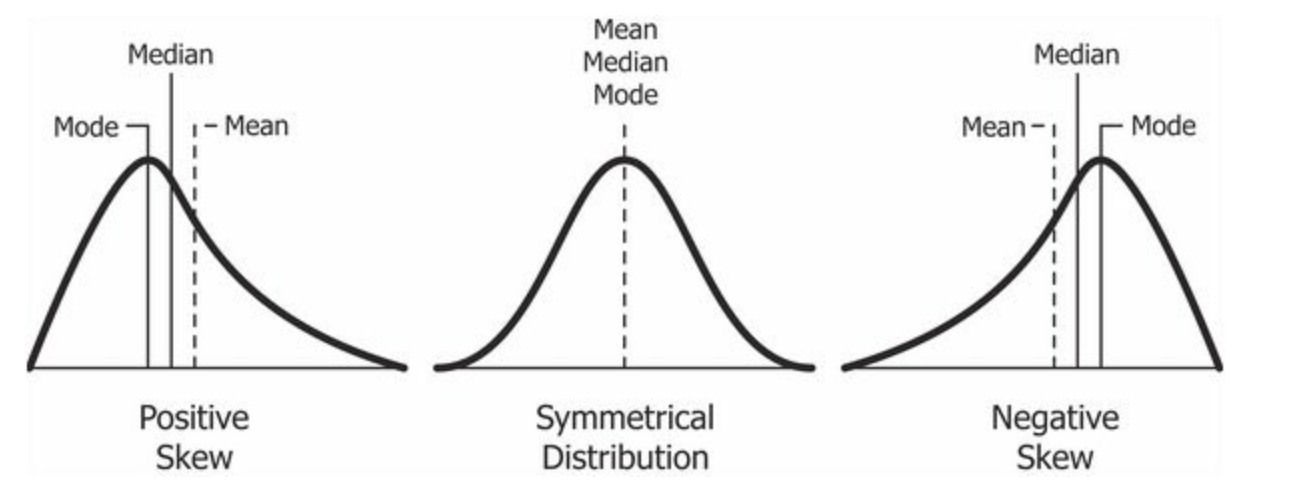
\includegraphics[scale=0.8]{lit_review/skewness.png}
      \caption{Skewness Visualisation}
      \label{skewness fig}
      \emph{Source: Wikipedia}
\end{figure}

\subsubsection{Kurtosis}

The kurtosis also measure 
\subsubsection{Z-Score}

\subsubsection{Correlation}

\subsubsection{P-Value}

\subsection{TODO: VAR / Causality Test}
TODO
%- main statistical measures
%- correlation 
%- statistical significance (look into durbin watson), hypothesis testing
%- F-statistic with p-value
%- unit root test
%- R\^2
%- granger causuality test
%- VAR ?
%- variance, z-score
